\documentclass[11pt]{article}

\usepackage[margin=1in]{geometry}
\usepackage{amsmath,amssymb,amsthm}
\usepackage{graphicx}
\usepackage{booktabs}
\usepackage{xcolor}
\usepackage{hyperref}
\usepackage{tikz}
\usetikzlibrary{positioning,arrows.meta}
\usepackage{float}
\usepackage{caption}

\newtheorem{theorem}{Theorem}
\newtheorem{definition}{Definition}
\newtheorem{example}{Example}

\title{\textbf{D2T-RNA: An Auditable Finite Controlled-Testing Prototype with a Negative Registered Evaluation and Fail-Closed RNA Data Qualification}}
\author{cunyuliu\\\small Zhejiang University\\\small \texttt{tylcy020509@qq.com}}
\date{\today}

\begin{document}
\maketitle

\begin{abstract}
\noindent D2T-RNA is an auditable software prototype for finite, non-adaptive categorical controlled testing: given a finite catalog of hypotheses, categorical observation actions with registered costs, and a fixed observation horizon, it computes exact separation/collision status, equal-prior Bayes average error, randomized minimax error, and cost-to-endpoint allocations, and emits independently reproducible certificates. We report three findings. First, a production audit corrected a central semantic defect: the discrete-certificate path had been silently dispatching to a convex-hull relaxation, and a single scalar had conflated equal-prior Bayes average error with randomized minimax error; the repaired interface separates these estimands, and the classical counterexamples ($1/4$ vs.\ $1/3$; $81/512$ vs.\ $81/337$) are now distinguished exactly. Second, a pre-registered synthetic evaluation on 20 frozen cells, with a Chernoff fixed-budget comparator and a frozen randomized-minimax endpoint, did not meet its pre-specified cost-reduction goal: the median relative cost difference is $0$, with $3$ of $20$ cells strictly cheaper and $17$ tied. A subsequent post-hoc search using an exact optimal solver yields definitional ``never-worse'' dominance and is therefore not a performance finding. Third, a fail-closed audit of seven RNA structure-probing scopes (ADD, glycine, miniTTR, SAM-III, RORC) shows that none qualifies for a real likelihood, an executable action, a real marginal cost, or independent experimental units; the real-data route is terminated for current data. The contribution is a limited, auditable finite controlled-testing prototype with an honest negative registered evaluation and a documented evidence boundary, not an RNA SOTA method.
\end{abstract}

\section{Introduction}\label{sec:intro}

Chemical structure probing generates nucleotide-resolution reactivity profiles of RNA. A natural ambition is to \emph{choose} future probes, constructs, and experiments so that the resulting data discriminate among competing structural hypotheses as cheaply and reliably as possible. Several lines of work formalize this ambition: controlled sensing for multihypothesis testing \cite{nitinawarat2013controlled}, fixed-horizon active hypothesis testing \cite{kartik2022fixed}, sequential active testing \cite{naghshvar2013active}, robust discrimination designs \cite{wiens2009robust}, and model-based rational design for sequencing-based RNA structure mapping \cite{aviran2014rational}. The present project (``D2T-RNA'') built a software prototype in this design space.

This preprint is a \emph{negative-result methods/software report}. It documents (i) what the prototype computes and what a production audit corrected; (ii) a pre-registered synthetic evaluation whose cost-reduction goal was \emph{not} met; and (iii) a fail-closed qualification of seven real RNA datasets showing that none currently supports real likelihood, action, cost, or independent-unit claims. We deliberately do not claim RNA SOTA, validated experiment design, or transferability.

A central theme is the distinction between \emph{formal certificate} and \emph{empirical validation}. A program can emit an exact, machine-checkable certificate for a finite problem while the underlying optimization objective is mis-specified, the method identity is mislabeled, or the data cannot support the intended statistical claim. The prototype's exact arithmetic and certificates are a strength; whether they constitute a scientifically useful experiment-design method is a separate, largely negative, question that this report addresses honestly.

\begin{figure}[H]\centering
% fig_evidence_flow.tikz — evidence/data flow and four-layer conclusion boundary
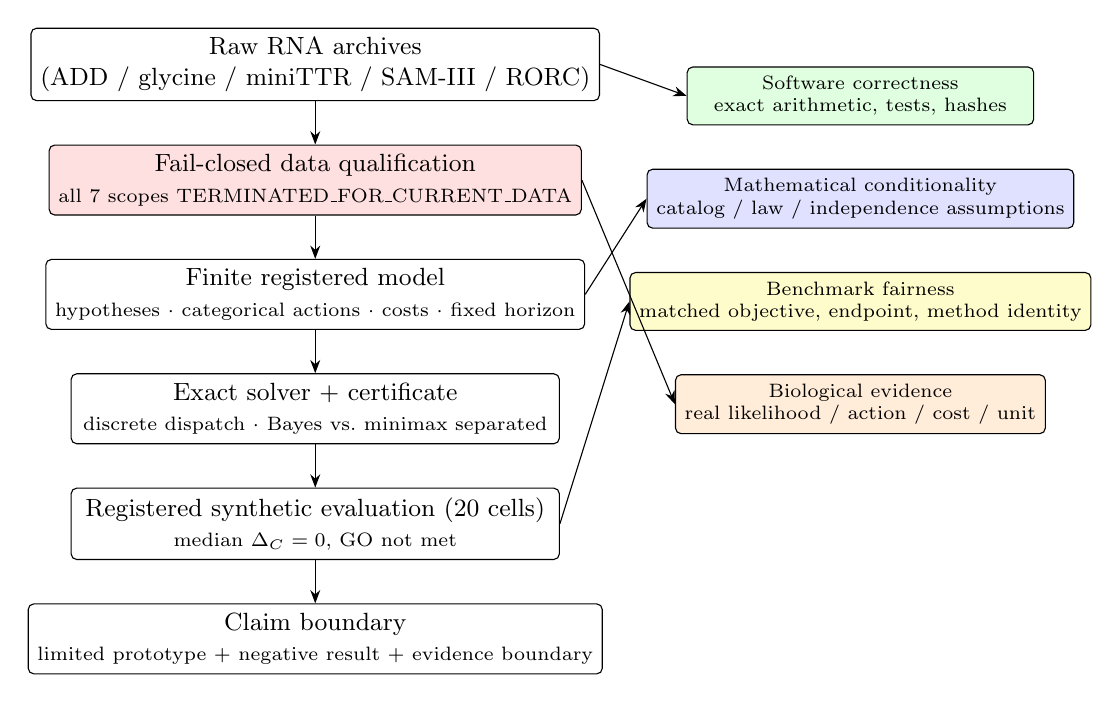
\begin{tikzpicture}[
  node distance=0.55cm,
  box/.style={draw, rounded corners=2pt, align=center, font=\small, minimum width=6.2cm, minimum height=0.85cm},
  layer/.style={draw, rounded corners=2pt, align=center, font=\scriptsize, minimum width=4.4cm, minimum height=0.7cm},
  ->, >=Stealth
]
  % data flow (left column)
  \node[box] (raw) {Raw RNA archives \\ (ADD / glycine / miniTTR / SAM-III / RORC)};
  \node[box, fill=red!12, below=of raw] (qual) {Fail-closed data qualification \\ {\scriptsize all 7 scopes TERMINATED\_FOR\_CURRENT\_DATA}};
  \node[box, below=of qual] (model) {Finite registered model \\ {\scriptsize hypotheses $\cdot$ categorical actions $\cdot$ costs $\cdot$ fixed horizon}};
  \node[box, below=of model] (solver) {Exact solver + certificate \\ {\scriptsize discrete dispatch $\cdot$ Bayes vs.\ minimax separated}};
  \node[box, below=of solver] (eval) {Registered synthetic evaluation (20 cells) \\ {\scriptsize median $\Delta_C = 0$, GO not met}};
  \node[box, below=of eval] (claim) {Claim boundary \\ {\scriptsize limited prototype + negative result + evidence boundary}};
  \draw[->] (raw) -- (qual);
  \draw[->] (qual) -- (model);
  \draw[->] (model) -- (solver);
  \draw[->] (solver) -- (eval);
  \draw[->] (eval) -- (claim);

  % four-layer conclusion boundary (right column)
  \node[layer, fill=green!12, right=1.1cm of raw, yshift=-0.4cm] (L1) {Software correctness \\ {\scriptsize exact arithmetic, tests, hashes}};
  \node[layer, fill=blue!12, below=of L1] (L2) {Mathematical conditionality \\ {\scriptsize catalog / law / independence assumptions}};
  \node[layer, fill=yellow!20, below=of L2] (L3) {Benchmark fairness \\ {\scriptsize matched objective, endpoint, method identity}};
  \node[layer, fill=orange!15, below=of L3] (L4) {Biological evidence \\ {\scriptsize real likelihood / action / cost / unit}};
  \draw[->] (raw.east) -- (L1.west);
  \draw[->] (model.east) -- (L2.west);
  \draw[->] (eval.east) -- (L3.west);
  \draw[->] (qual.east) -- (L4.west);
\end{tikzpicture}

\caption{Evidence/data flow (left) and the four-layer conclusion boundary (right). Software correctness, mathematical conditionality, benchmark fairness, and biological evidence are kept separate; a failure in any layer prevents the corresponding claim.}\label{fig:flow}
\end{figure}

\section{Finite Registered Controlled-Testing Problem}\label{sec:problem}

\subsection{Model}\label{sec:model}

The prototype operates on a finite, discrete, non-adaptive model:

\begin{itemize}
  \item a finite set of hypotheses $\Theta=\{\theta_0,\theta_1\}$ (binary case; the code also supports finite multi-state catalogs);
  \item a finite set of categorical actions $a\in\mathcal{A}$, each inducing an observation law $Q_a(\cdot\,|\,\theta)$;
  \item a fixed, non-adaptive horizon: the allocation $n=(n_a)_{a\in\mathcal{A}}$ with $\sum_a n_a \le B$ (budget) is chosen before any observation;
  \item a decision rule that maps the collected outcome vector to a hypothesis or to abstention;
  \item registered per-action costs $c_a$, so that cost-to-endpoint is a meaningful estimand.
\end{itemize}

This is a standard fixed-sample controlled-testing setup (e.g.\ \cite{nitinawarat2013controlled,kartik2022fixed}). We do \emph{not} claim new foundational theorems: the building blocks --- Chernoff information, likelihood-ratio tests, integer covering, linear programming, and Markov-basis enumeration --- are classical \cite{chernoff1972sequential,wald1945sequential,hoeffding1963probability,moret1985minimizing,diaconis1998algebraic}.

\subsection{Estimands}\label{sec:estimands}

Two risk estimands are distinguished throughout.

\begin{definition}[Equal-prior Bayes average error]\label{def:bayes}
With equal prior over $\theta_0,\theta_1$, the Bayes average error of a decision rule is
\[
\mathrm{BayesAvg}(\delta) \;=\; \tfrac12\Big(\Pr_{\theta_0}[\delta\neq\theta_0]+\Pr_{\theta_1}[\delta\neq\theta_1]\Big).
\]
\end{definition}

\begin{definition}[Randomized minimax error]\label{def:minimax}
A randomized decision rule randomizes over deterministic rules $\delta_r$ with weights $q_r$. Its worst-case error is
\[
\mathrm{Minimax}(\delta) \;=\; \max_{\theta} \sum_r q_r \Pr_{\theta}[\delta_r\neq \theta].
\]
The \emph{randomized minimax error} is the value of the resulting zero-sum game, minimized over randomized rules and maximized over hypotheses.
\end{definition}

A classical example separates the two estimands:

\begin{example}\label{ex:classic}
Let $\theta_0=(1,0)$ and $\theta_1=(\tfrac12,\tfrac12)$ be outcome distributions over two outcomes, with one observation ($n=1$). The equal-prior Bayes average error is $1/4$; the randomized minimax error is $1/3$. With four conditionally independent observations ($n=4$), the corresponding values for the $CA_{p1}$ cell are $81/512$ and $81/337$, respectively. These are verified exactly by the repaired interface (Section~\ref{sec:audit}).
\end{example}

\begin{theorem}[Definitional dominance]\label{thm:dominance}
Let $c^\ast$ be the minimum cost-to-endpoint over \emph{all} within-budget allocations that reach a fixed information/risk endpoint. Then for any strategy $S$ whose allocation is itself within-budget, $c^\ast \le c(S)$. In particular, an exact optimal solver is never worse than any such strategy.
\end{theorem}

Theorem~\ref{thm:dominance} is a definitional fact, not an empirical discovery; Section~\ref{sec:circular} explains why it cannot support a performance claim.

\section{What the Production Audit Corrected}\label{sec:audit}

The prototype went through a strict production audit. Three semantic defects were found and corrected.

\paragraph{Discrete/convex dispatch.}
The discrete-certificate path previously called a convex-hull linear program unconditionally. A counterexample with a discrete $\gamma_{\mathrm{L1}}=1/2$ but a convex-hull $\gamma=0$ was wrongly rejected by the production discrete entry point. The repaired `TheoremSpec` dispatches the `DISCRETE\_CATALOG` path to pure exact enumeration and never invokes the convex relaxation; unsupported combinations (`CONVEX\_HULL`, `PRODUCT\_TV`) fail closed with `UNSUPPORTED\_SPEC`. The discrete/convex counterexample is covered by production kill-tests.

\paragraph{Bayes vs.\ randomized minimax.}
A single scalar had been labelled `minimax\_error` while actually computing the equal-prior Bayes average error. The new result interface exposes both `bayes\_average\_error` and `randomized\_minimax\_error` as separate exact fractions. The classical counterexamples of Example~\ref{ex:classic} ($1/4$ vs.\ $1/3$; $81/512$ vs.\ $81/337$) are now reproduced exactly and covered by tests.

\paragraph{Method identity: oracle vs.\ deployable vs.\ comparator.}
Earlier comparative artifacts had used an exhaustive oracle as the ``D2T'' method, making ``never worse'' a definitional tautology. The audit enforces a three-way role separation --- oracle (reference/regret only), deployable (the actual algorithm), comparator --- and a consumer that rejects an oracle appearing in a win/tie/worse ranking.

\paragraph{Remaining gaps (disclosed).}
The certificate/checker is an \emph{experimental} API, not a complete end-to-end independent verification system: modifying `generator\_commit`, `generator\_tree`, or `verifier\_version` can still verify; values not in the registered catalog (or not even valid distributions) can still verify; and the certificate/checker is not wired into the production Phase 4/5 artifact chain. The constructive feasibility path is only locally repaired; the old information-only `FEASIBLE` path remains. These limitations are part of the honest evidence boundary.

\section{Negative Registered Synthetic Evaluation}\label{sec:negative}

\subsection{Protocol}\label{sec:protocol}

A pre-registered synthetic stress suite was frozen \emph{before} outcome access. The primary estimand is
\[
\Delta_{C,i} \;=\; \frac{\mathrm{cost}_{D2T,i}-\mathrm{cost}_{\mathrm{comparator},i}}{\mathrm{cost}_{\mathrm{comparator},i}},
\]
with the endpoint fixed at $1/10$ and the strongest comparator fixed at the Chernoff fixed-budget greedy \cite{chernoff1972sequential}. The pre-registered GO criterion requires a family-level median relative cost reduction of at least $10\%$.

\subsection{Result}\label{sec:result}

All $20$ frozen cells were solvable; none was withheld or failed. The result (exact fractions, from the committed artifact) is:

\begin{table}[H]\centering
\caption{Synthetic evaluation: method roles and outcome. Deployable = the actual fixed-budget solver; comparator = Chernoff greedy; oracle = reference only (not ranked).}\label{tab:synthetic}
\begin{tabular}{lcccl}
\toprule
Method role & \# cells & cost relation vs.\ comparator & median $\Delta_C$ & GO ($\geq 10\%$)? \\
\midrule
deployable (D2T) & 20 & $3$ lower / $17$ tie / $0$ higher & $0$ & no \\
comparator (Chernoff) & 20 & --- & --- & --- \\
oracle (reference) & 20 & regret only; not ranked & --- & --- \\
\bottomrule
\end{tabular}
\end{table}

\begin{figure}[H]\centering
% fig_delta_c.tikz — 20-cell v3 relative cost difference (median 0, GO not met)
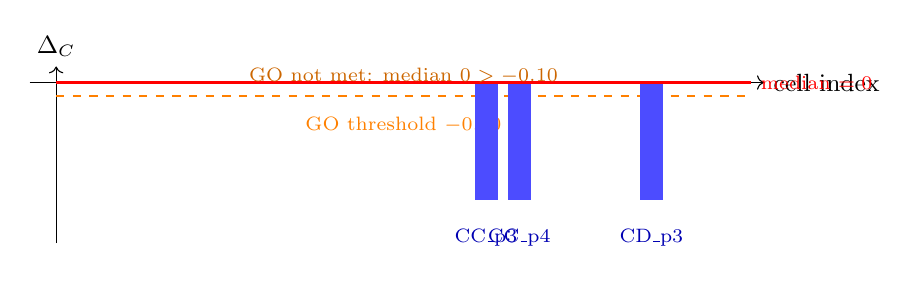
\begin{tikzpicture}[x=0.42cm,y=1.7cm]
  % axes
  \draw[->] (-0.8,0) -- (21.4,0) node[right,font=\small] {cell index};
  \draw[->] (0,-1.2) -- (0,0.12) node[above,font=\small] {$\Delta_C$};
  % GO threshold
  \draw[dashed,thick,orange] (0,-0.10) -- (21,-0.10)
        node[midway,below=4pt,font=\scriptsize,orange] {GO threshold $-0.10$};
  % all 20 cells at 0 (ties and the 3 lower cells share the 0 baseline)
  \foreach \i in {1,...,20} { \fill[gray!35] (\i-0.35,0) rectangle (\i+0.35,0); }
  % the 3 lower cells: CC_p3=13, CC_p4=14, CD_p3=18
  \foreach \i in {13,14,18} { \fill[blue!70] (\i-0.35,0) rectangle (\i+0.35,-0.875); }
  % median line at 0
  \draw[thick,red] (0,0) -- (21,0) node[right,font=\scriptsize,red] {median $= 0$};
  % labels for the 3 lower cells
  \node[font=\scriptsize,blue!70!black,anchor=north] at (13,-1.02) {CC\_p3};
  \node[font=\scriptsize,blue!70!black,anchor=north] at (14,-1.02) {CC\_p4};
  \node[font=\scriptsize,blue!70!black,anchor=north] at (18,-1.02) {CD\_p3};
  % GO not met annotation
  \node[font=\scriptsize,align=center,text=orange!80!black] at (10.5,0.05) {GO not met: median $0 > -0.10$};
\end{tikzpicture}

\caption{Per-cell relative cost difference $\Delta_C = (\mathrm{cost}_{D2T}-\mathrm{cost}_{\mathrm{chernoff}})/\mathrm{cost}_{\mathrm{chernoff}}$ on the 20 frozen cells. $3$ cells are strictly negative (cheaper), $17$ are ties at $0$, none is positive; the median is $0$, below the pre-registered $10\%$ reduction.}\label{fig:delta}
\end{figure}

The median $\Delta_C=0$ means the pre-registered GO was \emph{not} met. The registered evaluation therefore establishes only that the frozen implementation did not demonstrate a cost advantage over the frozen comparator on the frozen cells. This is a correct, fail-closed negative outcome.

\subsection{Objective mismatch}\label{sec:mismatch}

The result also exposes an objective mismatch: the deployed solver originally minimized equal-prior Bayes error under a fixed budget, whereas the final Track C estimand is \emph{cost-to-endpoint under randomized minimax}. The registered evaluation therefore proves ``the frozen implementation did not pass the frozen evaluation,'' not a universal negative about all possible D2T algorithms. We do not infer from it that no such algorithm could succeed.

\section{Why Exact-Oracle Superiority Is Circular}\label{sec:circular}

After the negative registration, a post-hoc ``method repair'' explored an exact optimal cost-to-endpoint solver over all within-budget allocations. Because it minimizes cost over the entire feasible set, Theorem~\ref{thm:dominance} applies: it is never worse than any within-budget strategy (in particular the Chernoff greedy), and strictly better exactly where the greedy is suboptimal.

This is mathematically true but scientifically vacuous as a \emph{performance} finding, for three reasons:

\begin{enumerate}
  \item \textbf{Definitional.} Any optimizer that minimizes over a set is never worse than a member of that set; no experiment is needed \cite{moret1985minimizing}. The ``never-worse'' is the definition of optimality, not an empirical advantage.
  \item \textbf{Catalog-constructed.} The hand-crafted ``method-distinguishing'' catalog was built \emph{after} observing the negative result, specifically so that the exact solver beats the greedy. A random-instance sweep shows the exact solver merely \emph{ties} the comparator (wins $0$); the strict wins exist only inside the constructed catalog.
  \item \textbf{Post-hoc selection.} Using a new catalog and a new solver to flip a pre-registered negative into ``GO met'' is outcome-informed instance selection, which the registration protocol explicitly forbids.
\end{enumerate}

Consequently, the post-hoc v5/v6 exploration is reported here only as an audit appendix (Section~\ref{sec:appendix}); it does not appear in the abstract, the main result, or any performance claim.

\section{Fail-Closed RNA Data Qualification}\label{sec:data}

The prototype intended to design real RNA experiments. Seven candidate scopes were audited under a fail-closed protocol: a scope is terminated for current data if any of raw per-replicate counts, an executable action, or a real marginal cost is missing, or if the independent statistical unit cannot be established.

\begin{table}[H]\centering
\caption{Seven-scope data-qualification matrix (full per-scope detail in the ancillary CSV). All scopes fail closed.}\label{tab:qual}
\resizebox{\textwidth}{!}{
\begin{tabular}{lccccccl}
\toprule
Scope & Raw counts & Replicate crosswalk & Calibrated likelihood & Executable action & Real cost & License receipt & Verdict \\
\midrule
ADD measured ($ADD71\_STD\_0001$) & no & no & no & no & no & unverified & terminated \\
ADD planning ($ADDAPO\_DCP\_0000$) & no & no & no & no & no & unverified & terminated \\
ADD Task6 ($ADDRSW\_SHP\_0003$) & no & no & no & no & no & unverified & terminated \\
Glycine ($BSUGLY\_DMS\_0013/14$) & no & merged only & no & no & no & unverified & terminated \\
miniTTR ($MTTR1\_MGTI\_0001$) & no & no & no & no & no & unverified & terminated \\
SAM-III ($GSE278422$) & no & no & no & no & no & unverified & terminated \\
RORC & no & no & no & no & no & unverified & terminated \\
\bottomrule
\end{tabular}}
\end{table}

Across all seven scopes the audit found: no per-replicate raw counts (only merged/normalized reactivity profiles); no verified biological-replicate crosswalk with an independent block unit; no calibrated count likelihood (clamping normalized reactivity is not a likelihood); no executable action with a real marginal cost; and no verified license receipt. Phase-2 sample-size numbers (e.g.\ $n=9806$) are count depth, not biological replicate $N$, and cannot support sample-size or repeat-count recommendations.

The conclusion is unambiguous and fail-closed: \emph{the real-data route is terminated for current data}. No quantitative certificate (gamma, absolute probability, reads/repeats, cost, or no-go) is derived from these scopes in this report.

\section{Lessons and Limitations}\label{sec:lessons}

\begin{itemize}
  \item \textbf{Software correctness is not empirical validation.} The prototype's exact arithmetic, certificates, and tests are reproducible; they do not establish that the optimized objective is the one an experimenter can act on, nor that the data support the intended estimand.
  \item \textbf{Mathematical conditionality.} Theorem~\ref{thm:dominance} and the exact computations hold under the registered catalog, action laws, and independence assumptions; whether real RNA satisfies them is unverified.
  \item \textbf{Benchmark fairness.} A fair comparison requires matched objectives, matched endpoints, matched budgets, and non-circular method identity. The registered negative result and the definitional-dominance caveat illustrate how easily each can fail.
  \item \textbf{Biological evidence.} None of the seven scopes can support biological claims. Real-data route: terminated.
  \item \textbf{Known software defects (disclosed).} The certificate/checker is not a full independent verification system; constructive feasibility is only locally repaired; two positive-path readiness regression tests are known to fail, so ``all tests pass'' is not claimed and no automated submission gate is asserted.
\end{itemize}

\section{Conclusion}\label{sec:conclusion}

D2T-RNA did not achieve RNA SOTA, validated real experiment design, or a synthetic cost-superiority result. It did produce a limited, auditable finite controlled-testing prototype: it distinguishes Bayes average error from randomized minimax error exactly; it dispatches discrete certificates without convex-hull contamination; and it fails closed on data that cannot support the intended claims.

The project is stopped. Its contribution is (i) a restricted prototype with explicit semantic repairs, (ii) an honest negative registered evaluation, and (iii) a documented evidence boundary for the real-data route. Archiving this negative result and its evidence boundary is the most reasonable --- and final --- scientific deliverable of the project.

\section{Appendix: Post-hoc Exploration (audit-only)}\label{sec:appendix}

For audit completeness we record the post-hoc exploration, \emph{not} as a result but as a warning example.

\paragraph{v5: cost-weighted myopic greedy.}
A greedy that adds, at each step, the unit action with the greatest marginal randomized-minimax reduction per unit cost. On the hand-crafted catalog it achieved a median $\Delta_C\approx-0.118$ (GO met on that catalog), but on a random-instance sweep it still had losses and an average $\Delta_C\approx+0.07$ --- a hidden weakness masked by the catalog.

\paragraph{v6: exact optimal solver.}
An exact solver over all within-budget allocations. By Theorem~\ref{thm:dominance} it is never worse than any within-budget comparator and ties the comparator on random instances (wins $0$); its strict wins are confined to the constructed catalog. The ``dominance theorem'' is the definition of optimality, and ``16/16 strict wins over Chernoff'' on a catalog built to make it win is circular. Per Section~\ref{sec:circular}, this does not appear in any main claim.

\paragraph{Classical counterexample.}
$P_0=(1,0)$, $P_1=(1/2,1/2)$, $n=1$: Bayes average $1/4$, randomized minimax $1/3$; $CA_{p1}$, $n=4$: $81/512$ vs.\ $81/337$. Both are reproduced exactly by the repaired interface.

\bibliographystyle{plain}
\bibliography{references}

\end{document}
